\subsubsection{Quản lý huy hiệu, xếp hạng các homestay}
\subsubsubsection{User Story}
\textit Từ kết quả rating,{Diamond Stay} sẽ quản lí huy hiệu và xếp hạng các homestay. Dựa trên cơ sở này, người dùng có thể dễ dàng biết được mức độ chuyên nghiệp cũng như chất lượng thực sự của homestay

\subsubsubsection{Mô tả các use case}
\begin{enumerate}[label=\textbf{(\alph*)}]
    \begin{figure}[!h]
        	\centering
        	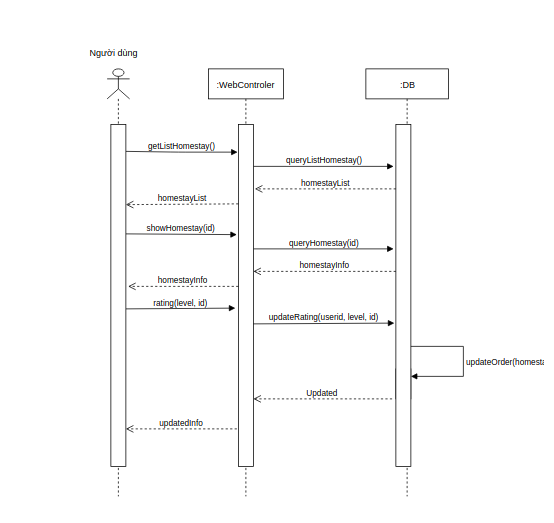
\includegraphics[width=13cm]{Image/tin-sequence-homstay-order.png}
        	\caption{Sequence Diagram cho usecase xếp hạng các homestay}
    \end{figure}
	\item \textbf{Usecase 3: Quản lý huy hiệu và xếp hạng các homestay.}
	\begin{center}
		\begin{longtable}{ | l |p{10cm}|}
			\hline
			\textbf{Tên usecase} & Quản lý huy hiệu và xếp hạng các homestay \\ \hline
			\textbf{Người tương tác} & Người dùng hệ thống \\ \hline   
			\textbf{Mô tả} &  Hệ thống tự động cập nhật huy hiệu và thứ hạng của nhà sau khi có 1 ratingmới của nhà xuất hiện. \\ \hline  
			\textbf{Người tạo:} \textit{Trần Ngọc Tín} & \textbf{Cập nhật lần cuối bởi:} \textit{Trần Ngọc Tín} \\ \hline
			\textbf{Ngày tạo:} \textit{22/03/2019} & \textbf{Lần cuối cập nhật:} \textit{30/03/2019} \\ \hline
			\textbf{Tiền điều kiện} &  Người dùng nào đó rating nhà. \\ \hline 
			\textbf{Hậu điều kiện} &  Thông tin về huy hiệu và thứ hạng của nhà đó được cập nhật \\ \hline 
			\textbf{Luồng cơ bản} & 
			\begin{enumerate}
		\item Người dùng rating nhà
		\item Hệ thống tính toán lại mức rating trung bình của nhà đó cũng như tổng số rating
		\item Hệ thống cập nhật lại huy hiệu cho nhà dựa theo mức rating trung bình và tổng số rating, chi tiết như sau:
		\begin{itemize}
		    \item Với nhà có tổng rating dưới 5: huy hiệu là "Nhà mới"
		    \item Với nhà đạt được tổng rating > 5 và <= 10: huy hiệu là "Nhà phổ biến"
		    \item Với nhà có tổng rating > 10, lúc này sẽ tính huy hiệu theo rating trung bình
		    \begin{itemize}
		        \item Với rating trung bình < 1: huy hiệu "Nhà quá tệ"
		        \item Với rating trung bình >= 1 và < 2: huy hiệu "Nhà tệ"
		        \item Với rating trung bình >= 2 và < 3: huy hiệu "Nhà tạm được"
		        \item Với rating trung bình >= 3 và < 4: huy hiệu "Nhà tốt"
		        \item Với rating trung bình >= 4 và <= 5: huy hiệu "Nhà tuyệt vời"
		    \end{itemize}
		\end{itemize}
		\item Hệ thống tính toán lại thứ tự ưu tiên của nhà theo mức rating trung bình mới, nhà nào có mức rating trung bình cao thì xếp hạng cao, nếu 2 nhà có mức rating trung bình bằng nhau thì dựa vào tổng số rating để xếp hạng, nhà nào có tổng rating cao hơn thì xếp hạng cao hơn
			\end{enumerate} \\ \hline
			\textbf{Luồng thay thế} & Không có \\ \hline
			\textbf{Ngoại lệ}  & Không có \\
			\hline
		\end{longtable}
	\end{center}
\end{enumerate}